\documentclass[11pt]{article}
\usepackage{freerbmt11}
\usepackage[utf8]{inputenc}
\usepackage{natbib}
\usepackage{times}
\usepackage{url}
\usepackage{latexsym}
\usepackage[pdftex]{graphicx}
\usepackage{listings}

\bibdata{ApertiumAWI.bib}

\title{Apertium Advanced Web Interface \\ 
A first step towards interactivity and language tools convergence}

\author{
Arnaud Vié \\ 
\\*
Informations Systems \\* Engineering \\
Grenoble INP - Ensimag \\
{\tt arnaud.vie@ensimag.fr}
\And 
Luis Villarejo Muñoz, \\*
{\bf Mireia Farrús Cabeceran} \\
Learning Technologies Office \\
Universitat Oberta de Catalunya \\ 
{\tt lvillarejo@uoc.edu,} \\* 
{\tt mfarrusc@uoc.edu} 
\And
Jimmy O'Regan \\
\\*
Eolaistriu Technologies \\
Thurles \\
Ireland \\
{\tt joregan@gmail.com}
}

\date{November 21th, 2010}

\begin{document}
\maketitle

\begin{abstract}
This document describes a project aimed at building a new web interface 
to the Apertium machine translation platform, including pre-editing and 
post-editing environments. It contains a description of the accomplished 
work on this project, as well as an overview of possible future work.
\end{abstract}

\section{Introduction}
One of the classic, and still open, tasks of Natural Language Processing 
(NLP) is Machine Translation (MT). Since its first steps, back in the 
1950s~\citep{Hutchins92b}, MT has increased its presence in several 
scenarios providing access to multilingual content. The number of MT 
initiatives has risen greatly in recent years, mainly in statistical MT, as 
a result of the availability of vast multilingual parallel texts, but also 
in rule-based MT, example-based MT or hybrid systems. 

One such example is the Apertium machine translation 
engine\footnote{http://www.apertium.org}. Apertium is a transfer-based MT 
platform which provides the engine, tools and data to perform translations 
between a large number of language pairs, available under the terms of 
the GNU General Public 
License (GNU GPL)\footnote{http://www.gnu.org/copyleft/gpl.html}, and is being 
developed by a community of users worldwide. 
It has been integrated in a wide variety of translation workflows both 
at public institutions like The Open University of 
Catalonia~\citep{Villarejo:09} and private institutions such as
Autodesk~\citep{Masselot10}. 

Apertium's basic design is based on the 
earlier Spanish--Catalan MT system 
interNOSTRUM\footnote{http://www.internostrum.com}~\citep{canals01b},
and the Spanish--Portuguese translator Traductor
Universia\footnote{http://traductor.universia.net}~\citep{garrido04}.
developed by the Transducens group at the University of Alicante. 

Apertium is designed to operate as a UNIX pipeline~\citep{mcilroy1978unix}: 
each component is implemented as a separate program, which reads and writes 
a simple text stream. Components can be added or removed as required: 
typical components in an Apertium pipeline include:
\begin{itemize}
\item A \emph{deformatter} which encapsulates the format information
 in the input as \emph{superblanks} that will then be seen
 as blanks between words by the rest of the modules.
\item A \emph{morphological analyser} which segments the text in
 surface forms (\emph{words}) and delivers, for each of them,
 one or more \emph{lexical forms} consisting of \emph{lemma},
 \emph{lexical category} and morphological inflection information.
\item A \emph{PoS tagger} which chooses the most
 likely lexical form corresponding to an ambiguous surface form.
\item A \emph{lexical transfer} module which reads each SL lexical
 form and delivers the corresponding target-language (TL) lexical
 form by looking it up in a bilingual dictionary.
\item A \emph{morphological generator} which delivers a TL surface
  form for each TL lexical form, by suitably inflecting it.
\item A \emph{post-generator} which performs orthographic operations
  such as contractions (e.g. Spanish \emph{del = de + el}) and
  apostrophations (e.g. Catalan \emph{l'institut = el + institut}).
\item A \emph{reformatter} which de-encapsulates any format
  information.
\end{itemize}

A complete description of the platform can be found in ~\cite{forcada09p}.

Despite the advances in MT, there has yet to be a system that can
produce a perfect translation. For the purpose of {\it assimilation},
or the understanding of text, MT can be sufficient; however, for the
purpose of {\it dissemination}, or the publication of translated
material, correction (post-editing) by a human editor is typically 
required. \cite{Doyon08} divides these edits into two main categories:
{\it Full Edits} (larger changes, mainly stylistic), and {\it Brief
Edits} (small changes, mainly syntactic).

Automating the process of post-editing is itself an active area of
research, both in SMT~\citep{Chin08}, and in rule-based MT.
\cite{llitjos04} describes a method of automatically refining rules
in a transfer-based system based on user feedback; however, the types
of edits permitted are restricted to Brief Edits, while for this work,
we aimed at allowing the editor full freedom to edit as they saw fit. 

\section{Overview}

The Apertium platform lacks one important aspect: the ability to get  
user feedback on the quality of the translation, in order to 
improve the translation process. 
Therefore, the initial aim of the project was to build a post-editing 
environment in which users may correct the translation they obtained, and 
that the changes they made may be logged by the system to benefit from 
that user's feedback.

With that goal in mind, we realised that a great number of the typical 
mistakes found in an automatically translated document are due to 
mistakes in the source document. 
Thus, the inclusion of automatic tools that can highlight to the user 
possible errors or perform efficiently certain repetitive tasks regarding 
the source document which could improve the translation process.

However, Apertium's web interface\footnote{Available on 
\url{http://www.apertium.org}} 
is fundamentally inadequate for such a task, as it takes care of the whole 
translation process at once. Here, it is necessary to pause before 
translation (for pre-editing) and just after the automatic translation 
(for post-editing) to enable the user to check for 
mistakes and correct them in both the source document and the translated 
output, with all tasks performed via the web interface to allow logging of 
the edits, hence it proved necessary to build a whole new interface, as 
well as a framework for future post-editing tools. 

This gave birth to the Apertium Advanced Web Interface (AWI) project.
As part of the Apertium project, it is available under the terms of the
GNU GPL, and hosted on Apertium's SVN
repository\footnote{http://apertium.svn.sourceforge.net/}.

\begin{figure*}[!ht]
  \caption{\label{CaptureOverallLayout} Overall interface layout}
     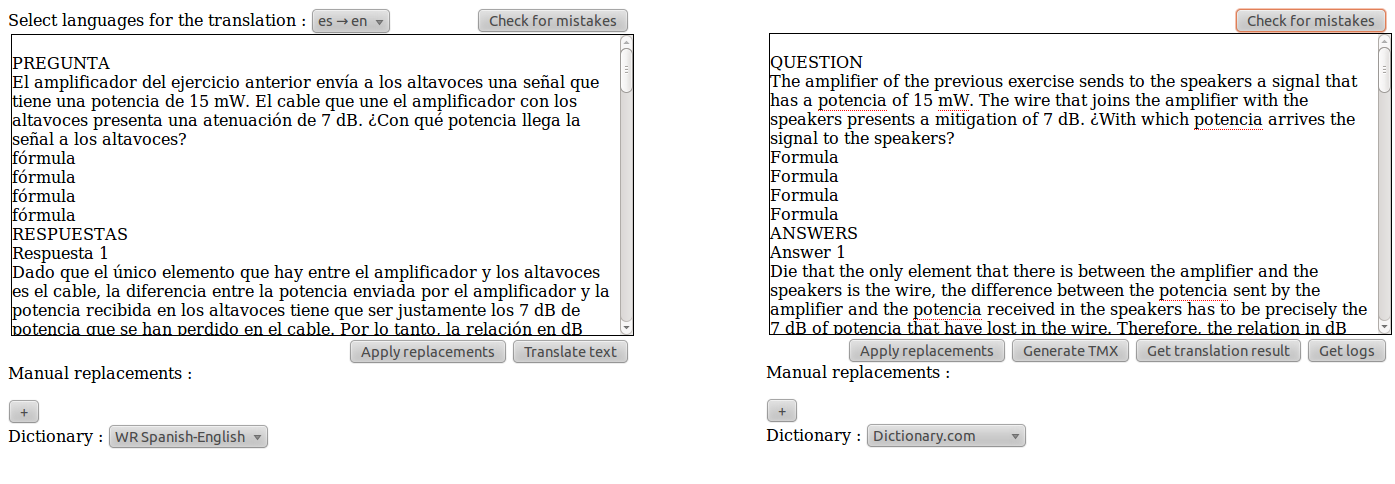
\includegraphics[width=\textwidth]{CaptureOverallLayout.png}
\end{figure*}

\section{Benefiting from user edits}

\subsection{Translation Memory generators and their limits}

A simple way, quite commonly used in the NLP community, to benefit from 
the translation's result is decomposing both source and generated texts 
in smaller elements, and then find the correspondance between them with 
an aligning algorithm. 
This Advanced Interface embeds such a tool, 
mALIGNa\footnote{http://align.sourceforge.net/}~\citep{Lipski08}, 
making it able to generate a Translation Memory (TM) of the 
result in the TMX format~\citep{tmx05}. 
A small example of such file is given below in Figure~\ref{TMXSample}.

\begin{figure}[!ht]
\caption{\label{TMXSample} Example of TMX file}
\begin{small}
\begin{verbatim}
<?xml version="1.0"?>
<tmx version="version 1.1">
<header 
  creationtool="Apertium TMX Builder">
</header>
<body>
<tu>
  <tuv xml:lang="en">
    <seg>This is a test</seg>
  </tuv>
  <tuv xml:lang="es">
    <seg>Esto es una prueba</seg>
  </tuv>
</tu>
<tu>
  <tuv xml:lang="en">
    <seg>This is test 3</seg>
  </tuv>
  <tuv xml:lang="es">
    <seg>Esto es prueba 3</seg>
  </tuv>
</tu>
</body>
</tmx>
\end{verbatim}
\end{small}
\end{figure}

Such a TM can then be reused by translation engines if they encounter 
the same elements later. 
Many engines allow for approximative matches to be considered as well, 
so that these memories be used in more different cases. 
Ideally, when Apertium has better support for TMX 
input\footnote{Currently, only a subset of TMX 1.1 is supported.} 
we could store 
this file locally as well to keep a corpus of completed translations 
and reuse it.

However, while being widely supported and quite simple to use, this 
approach also has a major drawback: it is virtually impossible to have 
it working on a lower level than complete sentences. 
Indeed, while most sentences retain punctuation, relative order and 
length throughout the translation -- making aligning sentences rather 
simple -- words don't. 
The order of words is frequently changed, a single word can be translated 
into several, and so on.

%//Insert illustration of the difference


\subsection{Text edit logging: different possibilities}

A different approach, allowing for more precise analysis, is to log the 
changes made by the user in the target text after the translation. 
This isn't directly reusable in other translation processes, but it can 
help language pair maintainers get an idea of the changes to make.
There are two main ways to envision this analysis.

The first is to compare the initial and final forms of the document. 
A simple diff utility can provide the shortest list of transformations 
leading from the source text to the result. 
If the user has only made small changes in the process, this should give 
out good results. However, important changes may result in it being 
difficult for the diff tool to located changed and unchanged portions 
of the text properly.

The second is to log events in real time. In other words, getting
information on the user edits at the precise moment they are made.
The main advantage of this approach is that some specific events can  
then be handled in a specific way. For example, it enables logging a  
global replacement as such, while a comparison between input and output  
texts would point out one difference for each occurrence of the  
replacement.   
This is the approach implemented in the Apertium AWI project.
 
The central point of this approach is therefore the need to be able to 
interpret a small event at the moment it occurs, in the web browser, in 
terms of an operation on words and sentences. 
Indeed, the web browser gives technical information about events in terms 
of affected document node and position inside of the node, that have to 
be converted to the linguistic information we wish to obtain. 
This is all the more complex as the text can be contained in a lot of 
different document nodes, due to the original document's formatting 
information.

\subsection{An interface between browser information and linguistic data}

To deal with that problem, this project relies on a text data structure, 
basically a sequence of sentences that all are a sequence of words, with 
information on the position of each word in the document.
A word in that structure is represented by the object containing the 
following properties:
\begin{itemize}
  \item The current text data of the word, that will change as edits 
  occur.
  \item The original text data of the word when it was loaded. This 
  won't change during editing.
  \item A reference to the sentence object containing this word
  \item A reference to the document node containing this word
  \item The position of the word inside of that node
  \item References to the previous and next words of the text
\end{itemize}

All the same, a sentence is represented as:
\begin{itemize}
  \item References to its first and last words
  \item References to the previous and next sentences
\end{itemize}

And the text object contains references to its first and last 
sentences and words.

This way, locating the word affected by an event is quite easy. It is 
also easy to get the context around a word - the neighboring words, or 
event the complete sentence it belongs to. 
The hard part is keeping that structure synchronised with the real text 
as the edition goes on, and that is what the logging\_lowlevel module 
of the project does. 
It is done by handling elementary operations, ie inserting or deleting 
a character, and determine the structural change to operate considering 
the properties of the said event.

\subsection{The log structure}

Now that we can get the information to log in a useful form, it is time 
to generate a proper log. 
The {\tt\small logging\_lowlevel} module will call functions from the logging module 
whenever a basic operation is being performed. 
These operations include adding, deleting or editing a word, as well as 
splitting and merging sentences (by inserting or deleting punctuation).
This logging module can then be written to handle these basic operations 
in any desired way; for now, its main job is to group events regarding 
the same entity.
For example, if the user deletes the word ``the'', three events would be 
sent by the lowlevel module: edited the word twice, and then deleted it. 
That is, the elementary events involved are three character deletions, 
where the first two leave a part of the word (hence a word edition report), 
whereas the last event deletes the only character of the word (hence a 
word deletion report). 
%You're repeating yourself here:
The logging module takes care of grouping all these elementary logs into 
one word deletion log, and so on.
Of course, that module could quite simply be changed to group the events 
in different ways, to output more of the context of an event, and so on, 
without changing the lowlevel module that does most of the work.


\section{Improving the user experience with the translation}

The second objective of this project was to provide a simple interface as 
well as to integrate convenient tools into it to help the user get an 
accurate translation.
The following tools were included:

\subsection{Formatted document handling}

The text editor is able to handle formatted documents through the 
{\tt\small apertium-unformat} and {\tt\small apertium-reformat} modules,
which replace the usual Apertium format handling tools.
Currently, it supports the ODF~\citep{odf06} format, notably used in the 
OpenOffice suite, but this can be extended to other formats.
Translating formatted documents changes only one aspect of the user 
interface: non-deletable characters (displayed as grey spaces at 
the moment, see Figure~\ref{CaptureCloseupFormatting}) appear in the 
text to represent the superblanks containing format information, so 
the user can make more accurate decisions on where words should be
placed in relation to their formatting.

\begin{figure}[!h]
  \caption{\label{CaptureCloseupFormatting} Example of formatting 
  artefacts}
     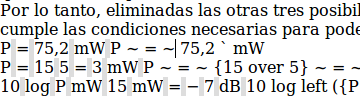
\includegraphics[width=\columnwidth]{CaptureCloseupFormatting.png}
\end{figure}

\subsection{Spell checking and Grammar checking}

The interface integrates the ability to check both input and output texts 
for mistakes. 
The interface provides a button ``Check for mistakes'' on top of each text 
editing field. 
When pressed, it runs spell checking and grammar checking on the text, 
in the language specified by the language pair selected for the 
translation, and underlines mistakes in different colours (red for 
spelling, blue for grammar). 
The user can then click on a mistake to see suggestions if they are 
available (Figure~\ref{CaptureCloseupSuggestions}) and select one; the 
description of a grammar error can also be seen when hovering over it, as 
shown in Figure~\ref{CaptureCloseupGrammarMistake}.

\begin{figure}[!h]
  \caption{\label{CaptureCloseupGrammarMistake} Grammar mistake 
  description}
     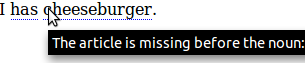
\includegraphics[width=\columnwidth]{CaptureCloseupGrammarMistake.png}
\end{figure}

\begin{figure}[!h]
  \caption{\label{CaptureCloseupSuggestions} Mistake correction 
  suggestions}
     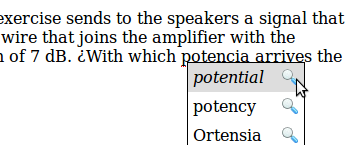
\includegraphics[width=\columnwidth]{CaptureCloseupSuggestions.png}
\end{figure}

All checking is done on the server, using AJAX to update the text in 
place. 
%This is where you should add more AJAX info!!
The server uses two main tools to provide the translation: 
Aspell~\citep{Atkinson04} for spell checking, and 
LanguageTool~\citep{Naber03} (in its server configuration) for 
grammar checking. 
The {\tt\small language.php} module written for this project handles 
reading and applying the output from both programs onto the text.

\subsection{Link to external dictionaries}

The user interface includes links to dictionaries next to all 
suggestions on mistakes, so that the user may easily find which one 
corresponds to the expected meaning. 
Whenever a dictionary for the language is available, a dictionary 
selection list is displayed under the text editing field, as shown in 
Figure~\ref{CaptureCloseupDictionaries}, and links to the right page 
on this dictionary included next to all suggestions. 
These links are visible in Figure~\ref{CaptureCloseupSuggestions} 
(page~\pageref{CaptureCloseupSuggestions}).
The interface selects available dictionaries by reading the OpenSearch~\citep{opensearch05} 
XML files organised in a folder on the server, making it easy to add 
new dictionaries.

\begin{figure}[!h]
  \caption{\label{CaptureCloseupDictionaries} External dictionary 
  selection}
     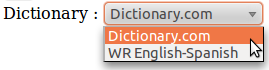
\includegraphics[width=\columnwidth]{CaptureCloseupDictionaries.png}
\end{figure}

\subsection{Search and replace}

The interface contains search and replace forms to instantly search for 
a word throughout the whole text and replace it, according to a specific 
pattern.
Available patterns are ``Case sensitive'', ``Case insensitive'' and 
``Apply source case''. 
This last mode runs a case insensitive search, executes a short 
case analysis on each match and tries to imitate the case on the 
replacement. 
For example, when an ``Apply source case'' replacement is set for ``herr'' 
to ``sir'', any occurrence of ``Herr'' will be replaced by ``Sir'', and so on.
This should allow speeding up the correction of long documents.


\section{Project conclusion and possible evolutions}

The main goals of this project have been reached, as it provides three 
major modules.

First, a basic interface for asynchronous translation, with document 
deformatting and reformatting and PHP Apertium interface on the server 
side, as well as a quick AJAX interface to update the text in place on 
client side.

Second, a set of tools to make translation more comfortable; mainly 
interfaces between the PHP script and other tools like LanguageTool and 
Aspell, and the ability to display their result in a clean way in the 
translation environment.

Third, tools to log the edits made by the user during the translation 
process, including TMX generation through mALIGNa and a real time edition 
logging engine.

\vspace{10pt}

However, there are still a few bugs happening during edition, depending 
on the browser used. 
The next step for the project obviously is to correct them and, if 
possible, make it more cross-browser compatible, as it has been mostly 
designed and tested on Firefox so far.

Another goal for the future is to make it smoother, to feel more like a 
usual translation environment, by integrating common user interaction 
events and removing the limitations of the current interface, such as 
the undeletable characters generated by the formatted document handling 
module and so on. 
Copy/Pasting have just been implemented, but there are still other 
limitations that could be frustrating for the user.

A quite important progress with benefiting from user input would be being 
able to reuse TMXs of successful translations when making a new one. 
Unfortunately, the Apertium TMX compiler isn't quite usable yet, but it 
should be possible to integrate an external tool like 
OmegaT\footnote{http://www.omegat.org/} to process part of the translation 
using the provided memories, before feeding the rest into Apertium.

At last, it could be useful to make this project more modular and 
adaptable. 
First, by reorganising the project’s source code as thematic modules: 
some people might want a simple and light translation interface 
without many tools, and some people may not care about translation 
logging. 
For this project to reach a wider use, reorganising it as more clearly 
separated and more configurable modules would be useful.
With the same idea, it would also be a good thing to leave more choice 
on what tools are to be used for all server-side tasks. 
For example, integration of After The 
Deadline\footnote{http://afterthedeadline.com/} as an alternative to 
LanguageTool could prove useful.

\section*{Acknowledgements}

Development for this project was funded by Google as part of the 
Google Summer of Code 2010 event; many thanks to Carol Smith and the 
GSoC team for organising it.

% Doing the author thing - silly to thank
%Special thanks to Jimmy O’Regan for his help with handling all the 
%external software involved as well as his useful advice, and to 
%Mireia Farrús Cabeceran for her regular feedback throughout the project.

Thanks to the LanguageTool developers, in particular Marcin Miłkowski 
for his help with solving a few bugs.

Thanks also to the anonymous reviewers for their comments.
% Mentioned in the article, no need to thank
%And at last, thanks to the developers of Aspell and mALIGNa, used as 
%external sofware for this project.

\bibliographystyle{apalike}
\bibliography{ApertiumAWI}

\end{document}

​